\chapter{傅里叶级数}

\section{傅里叶级数}

本章讨论在数学与工程技术中都有着广泛应用的一类函数项级数, 即由三角函数列所产生的三角级数.

\subsection{三角级数·正交函数系}

在科学实验与工程技术的某些现象中, 常会碰到一种周期运动. 最简单的周期运动, 可用正弦函数
\[
y = A\sin \left( {{\omega x} + \varphi }\right)  \tag{1}
\]
来描写. 由 (1) 所表达的周期运动也称为简谐振动,其中 \(A\) 为振幅, \(\varphi\) 为初相角, \(\omega\) 为角频率,于是简谐振动 \(y\) 的周期是 \(T = \frac{2\pi }{\omega }\) . 较为复杂的周期运动,则常是几个简谐振动
\[
{y}_{k} = {A}_{k}\sin \left( {{k\omega x} + {\varphi }_{k}}\right) ,\;k = 1,2,\cdots ,n
\]
的叠加
\[
y = \mathop{\sum }\limits_{{k = 1}}^{n}{y}_{k} = \mathop{\sum }\limits_{{k = 1}}^{n}{A}_{k}\sin \left( {{k\omega x} + {\varphi }_{k}}\right) . \tag{2}
\]
由于简谐振动 \({y}_{k}\) 的周期为 \(\frac{T}{k}\left( {T = \frac{2\pi }{\omega }}\right) ,k = 1,2,\cdots ,n\) ,所以函数 (2) 的周期为 \(T\) . 对无穷多个简谐振动进行叠加就得到函数项级数
\[
{A}_{0} + \mathop{\sum }\limits_{{n = 1}}^{\infty }{A}_{n}\sin \left( {{n\omega x} + {\varphi }_{n}}\right) . \tag{3}
\]
若级数 (3) 收敛, 则它所描述的是更为一般的周期运动现象. 对于级数 (3), 我们只要讨论 \(\omega  = 1\) (如果 \(\omega  \neq  1\) ,可用 \({\omega x}\) 代换 \(x\) ) 的情形. 由于
\[
\sin \left( {{nx} + {\varphi }_{n}}\right)  = \sin {\varphi }_{n}\cos {nx} + \cos {\varphi }_{n}\sin {nx},
\]
所以
\[
{A}_{0} + \mathop{\sum }\limits_{{n = 1}}^{\infty }{A}_{n}\sin \left( {{nx} + {\varphi }_{n}}\right)
\]
\[
= {A}_{0} + \mathop{\sum }\limits_{{n = 1}}^{\infty }\left( {{A}_{n}\sin {\varphi }_{n}\cos {nx} + {A}_{n}\cos {\varphi }_{n}\sin {nx}}\right) .
\]
 (3′)

记 \({A}_{0} = \frac{{a}_{0}}{2},{A}_{n}\sin {\varphi }_{n} = {a}_{n},{A}_{n}\cos {\varphi }_{n} = {b}_{n},\;n = 1,2,\cdots\) ,

则级数 \(\left( {3}^{\prime }\right)\) 可写成
\[
\frac{{a}_{0}}{2} + \mathop{\sum }\limits_{{n = 1}}^{\infty }\left( {{a}_{n}\cos {nx} + {b}_{n}\sin {nx}}\right) . \tag{4}
\]
它是由三角函数列 (也称为三角函数系)
\[
1,\cos x,\sin x,\cos {2x},\sin {2x},\cdots ,\cos {nx},\sin {nx},\cdots  \tag{5}
\]
所产生的一般形式的三角级数.

容易验证,若三角级数 (4) 收敛,则它的和一定是一个以 \({2\pi }\) 为周期的函数.

关于三角级数 (4) 的收敛性有如下定理.

%定理 15.1
\begin{theorem}{}{the:}

\end{theorem}
 若级数
\[
\frac{\left| {a}_{0}\right| }{2} + \mathop{\sum }\limits_{{n = 1}}^{\infty }\left( {\left| {a}_{n}\right|  + \left| {b}_{n}\right| }\right)
\]
收敛, 则级数 (4) 在整个数轴上绝对收敛且一致收敛.

%证
\begin{proof}

\end{proof}
对任何实数 \(x\) ,由于
\[
\left| {{a}_{n}\cos {nx} + {b}_{n}\sin {nx}}\right|  \leq  \left| {a}_{n}\right|  + \left| {b}_{n}\right| ,
\]
应用魏尔斯特拉斯 \(M\) 判别法 (定理 13.5) 就能推得本定理的结论.

为进一步研究三角级数 (4) 的收敛性, 我们先探讨三角函数系 (5) 具有哪些特性.

首先容易看出,三角函数系 (5) 中所有函数具有共同的周期 \({2\pi }\) .

其次,在三角函数系 (5) 中,任何两个不相同的函数的乘积在 \(\left\lbrack  {-\pi ,\pi }\right\rbrack\) 上的积分都等于零, 即
\[
{\int }_{-\pi }^{\pi }\cos {nx}\mathrm{\;d}x = {\int }_{-\pi }^{\pi }\sin {nx}\mathrm{\;d}x = 0, \tag{6}
\]
\[
\left. \begin{array}{l} {\int }_{-\pi }^{\pi }\cos {mx}\cos {nx}\mathrm{\;d}x = 0\;\left( {m \neq  n}\right) , \\  {\int }_{-\pi }^{\pi }\sin {mx}\sin {nx}\mathrm{\;d}x = 0\;\left( {m \neq  n}\right) , \\  {\int }_{-\pi }^{\pi }\cos {mx}\sin {nx}\mathrm{\;d}x = 0. \end{array}\right\}   \tag{7}
\]
而 (5) 中任何一个函数的平方在 \(\left\lbrack  {-\pi ,\pi }\right\rbrack\) 上的积分都不等于零,即
\[
\left. \begin{array}{l} {\int }_{-\pi }^{\pi }{\cos }^{2}{nx}\mathrm{\;d}x = {\int }_{-\pi }^{\pi }{\sin }^{2}{nx}\mathrm{\;d}x = \pi , \\  {\int }_{-\pi }^{\pi }{1}^{2}\mathrm{\;d}x = {2\pi }. \end{array}\right\}   \tag{8}
\]
若两个函数 \(\varphi\) 与 \(\psi\) 在 \(\left\lbrack  {a,b}\right\rbrack\) 上可积,且
\[
{\int }_{a}^{b}\varphi \left( x\right) \psi \left( x\right) \mathrm{d}x = 0,
\]
则称函数 \(\varphi\) 与 \(\psi\) 在 \(\left\lbrack  {a,b}\right\rbrack\) 上是正交的. 由此,三角函数系 (5) 在 \(\left\lbrack  {-\pi ,\pi }\right\rbrack\) 上具有正交性, 或称 (5) 是正交函数系.

\subsection{以 \({2\pi }\) 为周期的函数的傅里叶级数}

应用三角函数系 (5) 的正交性,我们讨论三角级数 (4) 的和函数 \(f\) 与级数 (4) 的系

数 \({a}_{0},{a}_{n},{b}_{n}\) 之间的关系.

%定理 15.2
\begin{theorem}{}{the:}

\end{theorem}
 若在整个数轴上
\[
f\left( x\right)  = \frac{{a}_{0}}{2} + \mathop{\sum }\limits_{{n = 1}}^{\infty }\left( {{a}_{n}\cos {nx} + {b}_{n}\sin {nx}}\right)  \tag{9}
\]
且等式右边级数一致收敛, 则有如下关系式:
\[
{a}_{n} = \frac{1}{\pi }{\int }_{-\pi }^{\pi }f\left( x\right) \cos {nx}\mathrm{\;d}x,\;n = 0,1,2,\cdots , \tag{10}
\]
\[
{b}_{n} = \frac{1}{\pi }{\int }_{-\pi }^{\pi }f\left( x\right) \sin {nx}\mathrm{\;d}x,\;n = 1,2,\cdots .
\]
%证
\begin{proof}

\end{proof}
由定理条件,函数 \(f\) 在 \(\left\lbrack  {-\pi ,\pi }\right\rbrack\) 上连续且可积. 对 (9) 式逐项积分得
\[
{\int }_{-\pi }^{\pi }f\left( x\right) \mathrm{d}x
\]
\[
= \frac{{a}_{0}}{2}{\int }_{-\pi }^{\pi }\mathrm{d}x + \mathop{\sum }\limits_{{n = 1}}^{\infty }\left( {{a}_{n}{\int }_{-\pi }^{\pi }\cos {nx}\mathrm{\;d}x + {b}_{n}{\int }_{-\pi }^{\pi }\sin {nx}\mathrm{\;d}x}\right) .
\]
由关系式 (6) 知, 上式右边括号内的积分都等于零. 所以
\[
{\int }_{-\pi }^{\pi }f\left( x\right) \mathrm{d}x = \frac{{a}_{0}}{2} \cdot  {2\pi } = {a}_{0}\pi ,
\]
即得
\[
{a}_{0} = \frac{1}{\pi }{\int }_{-\pi }^{\pi }f\left( x\right) \mathrm{d}x,
\]
现以 \(\cos {kx}\) 乘 (9) 式两边 ( \(k\) 为正整数),得
\[
f\left( x\right) \cos {kx} = \frac{{a}_{0}}{2}\cos {kx} + \mathop{\sum }\limits_{{n = 1}}^{\infty }\left( {{a}_{n}\cos {nx}\cos {kx} + {b}_{n}\sin {nx}\cos {kx}}\right) . \tag{11}
\]
从第十三章 §1 习题 4 知道,由级数 (9) 一致收敛,可推出级数 (11) 也一致收敛. 于是对级数 (11) 逐项求积, 有
\[
{\int }_{-\pi }^{\pi }f\left( x\right) \cos {kx}\mathrm{\;d}x
\]
\[
= \frac{{a}_{0}}{2}{\int }_{-\pi }^{\pi }\cos {kx}\mathrm{\;d}x + \mathop{\sum }\limits_{{n = 1}}^{\infty }\left( {{a}_{n}{\int }_{-\pi }^{\pi }\cos {nx}\cos {kx}\mathrm{\;d}x + {b}_{n}{\int }_{-\pi }^{\pi }\sin {nx}\cos {kx}\mathrm{\;d}x}\right) .
\]
由三角函数的正交性,右边除了以 \({a}_{k}\) 为系数的那一项积分
\[
{\int }_{-\pi }^{\pi }{\cos }^{2}{kx}\mathrm{\;d}x = \pi
\]
外, 其他各项积分都等于 0 , 于是得出
\[
{\int }_{-\pi }^{\pi }f\left( x\right) \cos {kx}\mathrm{\;d}x = {a}_{k}\pi \;\left( {k = 1,2,\cdots }\right) ,
\]
即
\[
{a}_{k} = \frac{1}{\pi }{\int }_{-\pi }^{\pi }f\left( x\right) \cos {kx}\mathrm{\;d}x\;\left( {k = 1,2,\cdots }\right) .
\]
同理,(9)式两边乘以 \(\sin {kx}\) ,并逐项求积,可得
\[
{b}_{k} = \frac{1}{\pi }{\int }_{-\pi }^{\pi }f\left( x\right) \sin {kx}\mathrm{\;d}x\;\left( {k = 1,2,\cdots }\right) .
\]
一般地说,若 \(f\) 是以 \({2\pi }\) 为周期且在 \(\left\lbrack  {-\pi ,\pi }\right\rbrack\) 上可积的函数,则按公式 (10) 计算出的 \({a}_{n}\) 和 \({b}_{n}\) 称为函数 \(f\) (关于三角函数系) 的傅里叶系数,以 \(f\) 的傅里叶系数为系数的三角级数 (9) 称为 \(f\) (关于三角函数系) 的傅里叶级数,记作
\[
f\left( x\right)  \sim  \frac{{a}_{0}}{2} + \mathop{\sum }\limits_{{n = 1}}^{\infty }\left( {{a}_{n}\cos {nx} + {b}_{n}\sin {nx}}\right) . \tag{12}
\]
这里记号“\~”表示上式右边是左边函数的傅里叶级数. 由定理 15.2 知道:若 (9) 式右边的三角级数在整个数轴上一致收敛于其和函数 \(f\) ,则此三角级数就是 \(f\) 的傅里叶级数,即此时 (12) 式中的记号 “ \(\sim\) ” 可换为等号. 然而,若从以 \({2\pi }\) 为周期且在 \(\left\lbrack  {-\pi ,\pi }\right\rbrack\) 上可积的函数 \(f\) 出发,按公式 (10) 求出其傅里叶系数并得到傅里叶级数 (12),这时还需讨论此级数是否收敛,以及如果收敛,是否收敛于 \(f\) 本身. 这就是下一段所要叙述的内容.

\subsection{收敛定理}

下面的定理称为傅里叶级数收敛定理.

%定理 15.3
\begin{theorem}{}{the:}

\end{theorem}
 若以 \({2\pi }\) 为周期的函数 \(f\) 在 \(\left\lbrack  {-\pi ,\pi }\right\rbrack\) 上按段光滑,则在每一点 \(x \in  \left\lbrack  {-\pi ,\pi }\right\rbrack  ,f\) 的傅里叶级数 (12) 收敛于 \(f\) 在点 \(x\) 的左、右极限的算术平均值,即
\[
\frac{f\left( {x + 0}\right)  + f\left( {x - 0}\right) }{2} = \frac{{a}_{0}}{2} + \mathop{\sum }\limits_{{n = 1}}^{\infty }\left( {{a}_{n}\cos {nx} + {b}_{n}\sin {nx}}\right) ,
\]
其中 \({a}_{n},{b}_{n}\) 为 \(f\) 的傅里叶系数.

下面先对定理中的某些概念作解释, 然后举例说明如何运用这个定理把函数展开成傅里叶级数. 关于收敛定理的证明将在 §3 中进行.

我们知道,若 \(f\) 的导函数在 \(\left\lbrack  {a,b}\right\rbrack\) 上连续,则称 \(f\) 在 \(\left\lbrack  {a,b}\right\rbrack\) 上光滑. 但若定义在 \(\left\lbrack  {a,b}\right\rbrack\) 上除了至多有有限个第一类间断点的函数 \(f\) 的导函数在 \(\left\lbrack  {a,b}\right\rbrack\) 上除了至多有限个点外都存在且连续,在这有限个点上导函数 \({f}^{\prime }\) 的左、右极限存在,则称 \(f\) 在 \(\left\lbrack  {a,b}\right\rbrack\) 上按段光滑.

根据上述定义,若函数 \(f\) 在 \(\left\lbrack  {a,b}\right\rbrack\) 上按段光滑,则有如下重要性质:

\({1}^{ \circ  }f\) 在 \(\left\lbrack  {a,b}\right\rbrack\) 上可积.

\({2}^{ \circ  }\) 在 \(\left\lbrack  {a,b}\right\rbrack\) 上每一点都存在 \(f\left( {x \pm  0}\right)\) ,且有
\[
\mathop{\lim }\limits_{{t \rightarrow  {0}^{ + }}}\frac{f\left( {x + t}\right)  - f\left( {x + 0}\right) }{t} = {f}^{\prime }\left( {x + 0}\right) , \tag{13}
\]
\[
\mathop{\lim }\limits_{{t \rightarrow  {0}^{ + }}}\frac{f\left( {x - t}\right)  - f\left( {x - 0}\right) }{-t} = {f}^{\prime }\left( {x - 0}\right) .
\]
\({3}^{ \circ  }\) 补充定义 \({f}^{\prime }\) 在 \(\left\lbrack  {a,b}\right\rbrack\) 上那些至多有限个不存在点上的值后 (仍记为 \({f}^{\prime }\) ), \({f}^{\prime }\) 在 \(\left\lbrack  {a,b}\right\rbrack\) 上可积.

从几何图形上讲,在区间 \(\left\lbrack  {a,b}\right\rbrack\) 上按段光滑函数,是由有限个光滑弧段所组成,它至多有有限个第一类间断点与角点 (图 15-1).

收敛定理指出, \(f\) 的傅里叶级数在点 \(x\) 处收敛于这一点上 \(f\) 的左、右极限的算术平均值 \(\frac{f\left( {x + 0}\right)  + f\left( {x - 0}\right) }{2}\) ; 而当 \(f\) 在点 \(x\) 连续时,则有 \(\frac{f\left( {x + 0}\right)  + f\left( {x - 0}\right) }{2} = f\left( x\right)\) ,即此时 \(f\) 的傅里叶级数收敛于 \(f\left( x\right)\) . 于是有下面推论.

推论 若 \(f\) 是以 \({2\pi }\) 为周期的连续函数,且在 \(\left\lbrack  {-\pi ,\pi }\right\rbrack\) 上按段光滑,则 \(f\) 的傅里叶级数在 \(\left( {-\infty , + \infty }\right)\) 上收敛于 \(f\) .

根据收敛定理的假设, \(f\) 是以 \({2\pi }\) 为周期的函数,所以系数公式 (10) 中的积分区间 \(\left\lbrack  {-\pi ,\pi }\right\rbrack\) 可以改为长度为 \({2\pi }\) 的任何区间,而不影响 \({a}_{n},{b}_{n}\) 的值:
\[
{a}_{n} = \frac{1}{\pi }{\int }_{c}^{c + {2\pi }}f\left( x\right) \cos {nx}\mathrm{\;d}x,n = 0,1,2,\cdots ,
\]
\[
{b}_{n} = \frac{1}{\pi }{\int }_{c}^{c + {2\pi }}f\left( x\right) \sin {nx}\mathrm{\;d}x,n = 1,2,\cdots ,
\]
(10′)

\begin{figure}
	\centering
	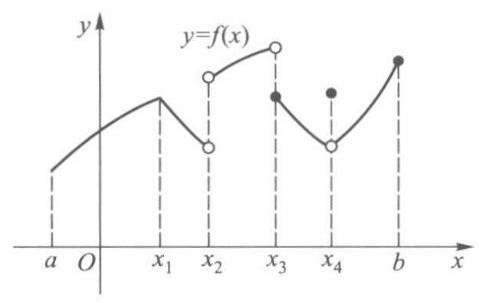
\includegraphics[width=.3\textwidth]{images/P105.jpg}
	\caption{图 $15-1$}
	\label{fig:P105}
\end{figure}

其中 \(c\) 为任何实数.

注意: 在具体讨论函数的傅里叶级数展开式时,常只给出函数 \(f\) 在 \(( - \pi ,\pi \rbrack\) (或 \(\lbrack  - \pi ,\pi ))\) 上的解析表达式,但读者应理解为它是定义在整个数轴上以 \({2\pi }\) 为周期的函数. 即在 \(( - \pi ,\pi \rbrack\) 以外的部分按函数在 \(( - \pi ,\pi \rbrack\) 上的对应关系作周期延拓. 如 \(f\) 为 \(( - \pi ,\pi \rbrack\) 上的解析表达式,那么周期延拓后的函数为
\[
\widehat{f}\left( x\right)  = \left\{  \begin{array}{l} f\left( x\right) ,x \in  ( - \pi ,\pi \rbrack , \\  f\left( {x - {2k\pi }}\right) ,x \in  (\left( {{2k} - 1}\right) \pi ,\left( {{2k} + 1}\right) \pi \rbrack ,\;k =  \pm  1, \pm  2,\cdots , \end{array}\right.
\]
如图 15-2 所示. 因此我们说函数 \(f\) 的傅里叶级数就是指函数 \(\widehat{f}\) 的傅里叶级数.

\begin{figure}
	\centering
	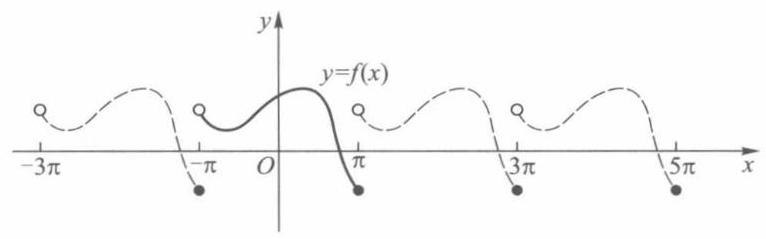
\includegraphics[width=.3\textwidth]{images/P106.jpg}
	\label{fig:P106}
\end{figure}

%例 1
\begin{example}

\end{example}
设
\[
f\left( x\right)  = \left\{  \begin{array}{ll} x, & 0 \leq  x \leq  \pi , \\  0, &  - \pi  < x < 0, \end{array}\right.
\]
求 \(f\) 的傅里叶级数展开式.

%解
\begin{solution}

\end{solution}
函数 \(f\) 及其周期延拓后的图像如图 15-3 所示. 显然 \(f\) 是按段光滑的,故由定理 15.3 (收敛定理), 它可以展开成傅里叶级数. 由于
\[
{a}_{0} = \frac{1}{\pi }{\int }_{-\pi }^{\pi }f\left( x\right) \mathrm{d}x = \frac{1}{\pi }{\int }_{0}^{\pi }x\mathrm{\;d}x = \frac{\pi }{2}.
\]
\begin{figure}
	\centering
	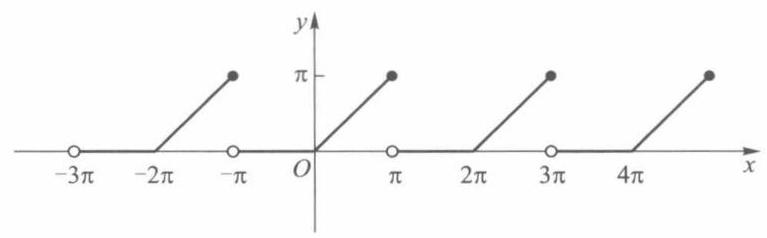
\includegraphics[width=.3\textwidth]{images/P107.jpg}
	\caption{图 $15-3$}
	\label{fig:P107}
\end{figure}

当 \(n \geq  1\) 时,
\[
{a}_{n} = \frac{1}{\pi }{\int }_{-\pi }^{\pi }f\left( x\right) \cos {nx}\mathrm{\;d}x = \frac{1}{\pi }{\int }_{0}^{\pi }x\cos {nx}\mathrm{\;d}x
\]
\[
= {\left. \frac{1}{n\pi }x\sin nx\right| }_{0}^{\pi } - {\left. \frac{1}{n\pi }{\int }_{0}^{\pi }\sin nx\mathrm{\;d}x = \frac{1}{{n}^{2}\pi }\cos nx\right| }_{0}^{\pi }
\]
\[
= \frac{1}{{n}^{2}\pi }\left( {\cos {n\pi } - 1}\right)  = \left\{  \begin{array}{ll}  - \frac{2}{{n}^{2}\pi }, & \text{ 当 }n\text{ 为奇数时, } \\  0, & \text{ 当 }n\text{ 为偶数时, } \end{array}\right.
\]
\[
{b}_{n} = \frac{1}{\pi }{\int }_{-\pi }^{\pi }f\left( x\right) \sin {nx}\mathrm{\;d}x = \frac{1}{\pi }{\int }_{0}^{\pi }x\sin {nx}\mathrm{\;d}x
\]
\[
=  - {\left. \frac{1}{n\pi }x\cos nx\right| }_{0}^{\pi } + \frac{1}{n\pi }{\int }_{0}^{\pi }\cos {nx}\mathrm{\;d}x
\]
\[
= {\left. \frac{{\left( -1\right) }^{n + 1}}{n} + \frac{1}{{n}^{2}\pi }\sin nx\right| }_{0}^{\pi }
\]
\[
= \frac{{\left( -1\right) }^{n + 1}}{n}\text{ . }
\]
所以在开区间 \(\left( {-\pi ,\pi }\right)\) 上,
\[
f\left( x\right)  = \frac{\pi }{4} - \left( {\frac{2}{\pi }\cos x - \sin x}\right)  - \frac{1}{2}\sin {2x} - \left( {\frac{2}{9\pi }\cos {3x} - \frac{1}{3}\sin {3x}}\right)  - \cdots .
\]
在 \(x =  \pm  \pi\) 时,上式右边收敛于
\[
\frac{f\left( {\pi  - 0}\right)  + f\left( {-\pi  + 0}\right) }{2} = \frac{\pi  + 0}{2} = \frac{\pi }{2}.
\]
于是,在 \(\left\lbrack  {-\pi ,\pi }\right\rbrack\) 上 \(f\) 的傅里叶级数的图像如图 15-4 所示 (注意它与图 15-3 的差别).

\begin{figure}
	\centering
	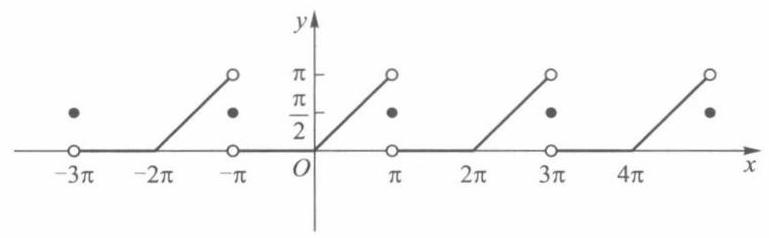
\includegraphics[width=.3\textwidth]{images/P108.jpg}
	\caption{图 $15-4$}
	\label{fig:P108}
\end{figure}

%例 2
\begin{example}

\end{example}
把下列函数展开成傅里叶级数:
\[
f\left( x\right)  = \left\{  \begin{array}{ll} {x}^{2}, & 0 < x < \pi , \\  0, & x = \pi , \\   - {x}^{2}, & \pi  < x \leq  {2\pi }. \end{array}\right.
\]
%解
\begin{solution}

\end{solution}
\(f\) 及其周期延拓的图形如图 15-5 所示. 显然 \(f\) 是按段光滑的,因此可以展开成傅里叶级数.

在 \(\left( {10}^{\prime }\right)\) 式中令 \(c = 0\) 来计算傅里叶系数如下:

\begin{figure}
	\centering
	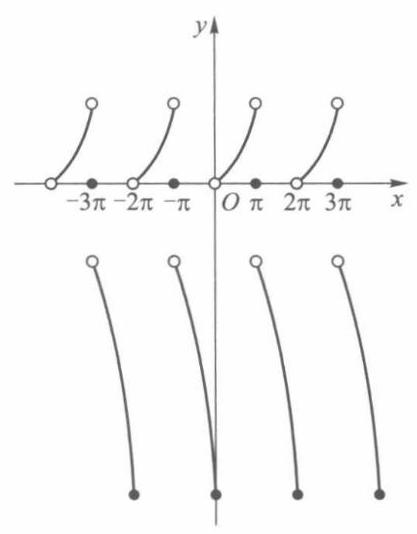
\includegraphics[width=.3\textwidth]{images/P109.jpg}
	\caption{图 $15-5$}
	\label{fig:P109}
\end{figure}
\[
{a}_{0} = \frac{1}{\pi }{\int }_{0}^{2\pi }f\left( x\right) \mathrm{d}x = \frac{1}{\pi }{\int }_{0}^{\pi }{x}^{2}\mathrm{\;d}x + \frac{1}{\pi }{\int }_{\pi }^{2\pi }\left( {-{x}^{2}}\right) \mathrm{d}x = \frac{{\pi }^{2}}{3} - \frac{7{\pi }^{2}}{3} =  - 2{\pi }^{2},
\]
\[
{a}_{n} = \frac{1}{\pi }{\int }_{0}^{2\pi }f\left( x\right) \cos {nx}\mathrm{\;d}x = \frac{1}{\pi }{\int }_{0}^{\pi }{x}^{2}\cos {nx}\mathrm{\;d}x + \frac{1}{\pi }{\int }_{\pi }^{2\pi }\left( {-{x}^{2}}\right) \cos {nx}\mathrm{\;d}x
\]
\[
= {\left. \frac{1}{\pi }\left\lbrack  \left( \frac{{x}^{2}}{n} - \frac{2}{{n}^{3}}\right) \sin nx + \frac{2x}{{n}^{2}}\cos nx\right\rbrack  \right| }_{0}^{\pi } - {\left. \frac{1}{\pi }\left\lbrack  \left( \frac{{x}^{2}}{n} - \frac{2}{{n}^{3}}\right) \sin nx + \frac{2x}{{n}^{2}}\cos nx\right\rbrack  \right| }_{\pi }^{2\pi }
\]
\[
= \frac{4}{{n}^{2}}\left\lbrack  {{\left( -1\right) }^{n} - 1}\right\rbrack  \text{ , }
\]
\[
{b}_{n} = \frac{1}{\pi }{\int }_{0}^{2\pi }f\left( x\right) \sin {nx}\mathrm{\;d}x = \frac{1}{\pi }{\int }_{0}^{\pi }{x}^{2}\sin {nx}\mathrm{\;d}x + \frac{1}{\pi }{\int }_{\pi }^{2\pi }\left( {-{x}^{2}}\right) \sin {nx}\mathrm{\;d}x
\]
\[
= {\left. \frac{1}{\pi }\left\lbrack  \left( -\frac{{x}^{2}}{n} + \frac{2}{{n}^{3}}\right) \cos nx + \frac{2x}{{n}^{2}}\sin nx\right\rbrack  \right| }_{0}^{\pi } - {\left. \frac{1}{\pi }\left\lbrack  \left( -\frac{{x}^{2}}{n} + \frac{2}{{n}^{3}}\right) \cos nx + \frac{2x}{{n}^{2}}\sin nx\right\rbrack  \right| }_{\pi }^{2\pi }
\]
\[
= \frac{2}{\pi }\left\{  {\frac{{\pi }^{2}}{n} + \left( {\frac{{\pi }^{2}}{n} - \frac{2}{{n}^{3}}}\right) \left\lbrack  {1 - {\left( -1\right) }^{n}}\right\rbrack  }\right\}  .
\]
所以当 \(x \in  \left( {0,\pi }\right)  \cup  \left( {\pi ,{2\pi }}\right)\) 时,
\[
f\left( x\right)  =  - {\pi }^{2} + \mathop{\sum }\limits_{{n = 1}}^{\infty }\left\{  {\frac{4}{{n}^{2}}\left\lbrack  {{\left( -1\right) }^{n} - 1}\right\rbrack  \cos {nx} + \frac{2}{\pi }\left\lbrack  {\frac{{\pi }^{2}}{n} + \left( {\frac{{\pi }^{2}}{n} - \frac{2}{{n}^{3}}}\right) \left( {1 - {\left( -1\right) }^{n}}\right) }\right\rbrack  \sin {nx}}\right\}
\]
\[
=  - {\pi }^{2} - 8\left( {\cos x + \frac{1}{{3}^{2}}\cos {3x} + \frac{1}{{5}^{2}}\cos {5x} + \cdots }\right)  + \frac{2}{\pi }\left\{  {\left( {3{\pi }^{2} - 4}\right) \sin x + }\right.
\]
\[
\left. {\frac{{\pi }^{2}}{2}\sin {2x} + \left( {\frac{3{\pi }^{2}}{3} - \frac{4}{{3}^{3}}}\right) \sin {3x} + \frac{{\pi }^{2}}{4}\sin {4x} + \cdots }\right\}  \text{ . }
\]
当 \(x = \pi\) 时,由于
\[
\frac{f\left( {\pi  - 0}\right)  + f\left( {\pi  + 0}\right) }{2} = 0,
\]
所以
\[
0 =  - {\pi }^{2} + 8\left( {\frac{1}{{1}^{2}} + \frac{1}{{3}^{2}} + \frac{1}{{5}^{2}} + \cdots }\right) . \tag{14}
\]
当 \(x = 0\) 或 \({2\pi }\) 时,由于
\[
\frac{1}{2}\left( {f\left( {0 - 0}\right)  + f\left( {0 + 0}\right) }\right)  = \frac{1}{2}\left( {-4{\pi }^{2} + 0}\right)  =  - 2{\pi }^{2},
\]
因此
\[
- 2{\pi }^{2} =  - {\pi }^{2} - 8\left( {\frac{1}{{1}^{2}} + \frac{1}{{3}^{2}} + \frac{1}{{5}^{2}} + \cdots }\right) . \tag{15}
\]
由 (14) 式或 (15) 式都可得出
\[
\frac{{\pi }^{2}}{8} = \frac{1}{{1}^{2}} + \frac{1}{{3}^{2}} + \frac{1}{{5}^{2}} + \cdots .
\]
%例 3
\begin{example}

\end{example}
在电子技术中经常用到矩形波, 用傅里叶级数展开后, 就可以将矩形波看成一系列不同频率的简谐振动的叠加, 在电工学中称为谐波分析。设 \(f\left( x\right)\) 是周期为 \({2\pi }\) 的矩形波函数 (图 15-6),在 \(\lbrack  - \pi ,\pi )\) 上的表达式为
\[
f\left( x\right)  = \left\{  \begin{matrix}  - \frac{\pi }{4}, &  - \pi  \leq  x < 0, \\  0, & x = 0, \\  \frac{\pi }{4}, & 0 < x < \pi . \end{matrix}\right.
\]
\begin{figure}
	\centering
	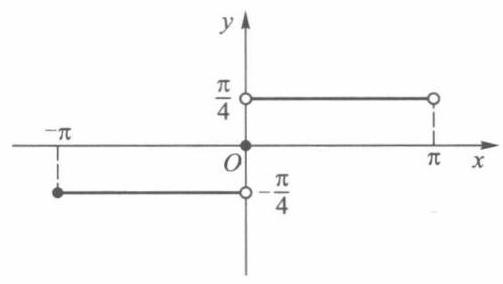
\includegraphics[width=.3\textwidth]{images/P110.jpg}
	\caption{图 $15-6$}
	\label{fig:P110}
\end{figure}

求该矩形波函数的傅里叶展开式.

%解
\begin{solution}

\end{solution}
由于 \(f\left( x\right)\) 在 \(\left( {-\pi ,\pi }\right)\) 上是奇函数,所以
\[
{a}_{0} = \frac{1}{\pi }{\int }_{-\pi }^{\pi }f\left( x\right) \mathrm{d}x = 0,
\]
\[
{a}_{n} = \frac{1}{\pi }{\int }_{-\pi }^{\pi }f\left( x\right) \cos {nx}\mathrm{\;d}x = 0,
\]
\[
{b}_{n} = \frac{1}{\pi }{\int }_{-\pi }^{\pi }f\left( x\right) \sin {nx}\mathrm{\;d}x = \frac{2}{\pi }{\int }_{0}^{\pi }\frac{\pi }{4}\sin {nx}\mathrm{\;d}x = \frac{1}{2n}\left\lbrack  {1 - {\left( -1\right) }^{n}}\right\rbrack  .
\]
于是当 \(x \neq  {k\pi },k = 0, \pm  1, \pm  2,\cdots\) 时,
\[
f\left( x\right)  = \sin x + \frac{1}{3}\sin {3x} + \cdots  + \frac{1}{{2n} - 1}\sin \left( {{2n} - 1}\right) x + \cdots ;
\]
当 \(x = {k\pi },k = 0, \pm  1, \pm  2,\cdots\) 时,级数收敛于 0 (实际上级数每一项都为 0 ). 其收敛过程如图 15-7 所示.

\begin{figure}
	\centering
	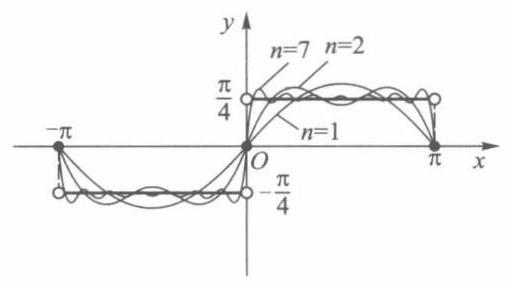
\includegraphics[width=.3\textwidth]{images/P111.jpg}
	\caption{图 $15-7$}
	\label{fig:P111}
\end{figure}

\subsection{习题 15.1}

1. 在指定区间上把下列函数展开成傅里叶级数:

( 1 ) \(f\left( x\right)  = x\) ,( i ) \(- \pi  < x < \pi\) ,( ii ) \(0 < x < {2\pi }\) ;

(2) \(f\left( x\right)  = {x}^{2}\) ,(i) \(- \pi  < x < \pi\) ,(ii) \(0 < x < {2\pi }\) ;

(3) \(f\left( x\right)  = \left\{  {\begin{array}{ll} {ax}, &  - \pi  < x \leq  0, \\  {bx}, & 0 < x < \pi  \end{array}\;\left( {a \neq  b,a \neq  0,b \neq  0}\right) }\right.\) .

2. 设 \(f\) 是以 \({2\pi }\) 为周期的可积函数,证明对任何实数 \(c\) ,有
\[
{a}_{n} = \frac{1}{\pi }{\int }_{c}^{c + {2\pi }}f\left( x\right) \cos {nx}\mathrm{\;d}x = \frac{1}{\pi }{\int }_{-\pi }^{\pi }f\left( x\right) \cos {nx}\mathrm{\;d}x,n = 0,1,2,\cdots ,
\]
\[
{b}_{n} = \frac{1}{\pi }{\int }_{c}^{c + {2\pi }}f\left( x\right) \sin {nx}\mathrm{\;d}x = \frac{1}{\pi }{\int }_{-\pi }^{\pi }f\left( x\right) \sin {nx}\mathrm{\;d}x,n = 1,2,\cdots .
\]
3. 把函数
\[
f\left( x\right)  = \left\{  \begin{matrix}  - \frac{\pi }{4}, &  - \pi  < x < 0, \\  \frac{\pi }{4}, & 0 \leq  x < \pi  \end{matrix}\right.
\]
展开成傅里叶级数, 并由它推出

(1) \(\frac{\pi }{4} = 1 - \frac{1}{3} + \frac{1}{5} - \frac{1}{7} + \cdots\) ;

(2) \(\frac{\pi }{3} = 1 + \frac{1}{5} - \frac{1}{7} - \frac{1}{11} + \frac{1}{13} + \frac{1}{17} + \cdots\) ;

(3) \(\frac{\sqrt{3}}{6}\pi  = 1 - \frac{1}{5} + \frac{1}{7} - \frac{1}{11} + \frac{1}{13} - \frac{1}{17} + \cdots\) .

4. 设函数 \(f\left( x\right)\) 满足条件 \(f\left( {x + \pi }\right)  =  - f\left( x\right)\) . 问此函数在 \(\left( {-\pi ,\pi }\right)\) 上的傅里叶级数具有什么特性.

5. 设函数 \(f\left( x\right)\) 满足条件 \(f\left( {x + \pi }\right)  = f\left( x\right)\) . 问此函数在 \(\left( {-\pi ,\pi }\right)\) 上的傅里叶级数具有什么特性.

6. 试证函数系 \(\cos {nx},n = 0,1,2,\cdots\) 和 \(\sin {nx},n = 1,2,\cdots\) 都是 \(\left\lbrack  {0,\pi }\right\rbrack\) 上的正交函数系,但它们合起来的 (5) 式不是 \(\left\lbrack  {0,\pi }\right\rbrack\) 上的正交函数系.

7. 求下列函数的傅里叶级数展开式:

(1) \(f\left( x\right)  = \frac{\pi  - x}{2},0 < x < {2\pi }\) ;

(2) \(f\left( x\right)  = \sqrt{1 - \cos x}, - \pi  \leq  x \leq  \pi\) ;

(3) \(f\left( x\right)  = a{x}^{2} + {bx} + c\) ,(i) \(0 < x < {2\pi }\) ,(ii) \(- \pi  < x < \pi\) ;

(4) \(f\left( x\right)  = \operatorname{ch}x, - \pi  < x < \pi\) ;

(5) \(f\left( x\right)  = \operatorname{sh}x, - \pi  < x < \pi\) .

8. 求函数 \(f\left( x\right)  = \frac{1}{12}\left( {3{x}^{2} - {6\pi x} + 2{\pi }^{2}}\right) ,0 < x < {2\pi }\) 的傅里叶级数展开式,并应用它推出 \(\frac{{\pi }^{2}}{6} = \sum \frac{1}{{n}^{2}}\) .

9. 设 \(f\) 为 \(\left\lbrack  {-\pi ,\pi }\right\rbrack\) 上的光滑函数,且 \(f\left( {-\pi }\right)  = f\left( \pi \right) .{a}_{n},{b}_{n}\) 为 \(f\) 的傅里叶系数, \({a}_{n}^{\prime },{b}_{n}^{\prime }\) 为 \(f\) 的导函数 \({f}^{\prime }\) 的傅里叶系数. 证明:
\[
{a}_{0}^{\prime } = 0,\;{a}_{n}^{\prime } = n{b}_{n},\;{b}_{n}^{\prime } =  - n{a}_{n}\;\left( {n = 1,2,\cdots }\right) .
\]
10. 证明: 若三角级数
\[
\frac{{a}_{0}}{2} + \mathop{\sum }\limits_{{n = 1}}^{\infty }\left( {{a}_{n}\cos {nx} + {b}_{n}\sin {nx}}\right)
\]
中的系数 \({a}_{n},{b}_{n}\) 满足关系
\[
\mathop{\sup }\limits_{n}\left\{  {\left| {{n}^{3}{a}_{n}}\right| ,\left| {{n}^{3}{b}_{n}}\right| }\right\}   \leq  M,
\]
\(M\) 为常数,则上述三角级数收敛,且其和函数具有连续的导函数.

\section{以 \({2l}\) 为周期的函数的展开式}

在上节的收敛定理中,假设函数 \(f\) 是以 \({2\pi }\) 为周期的,或是定义在 \(( - \pi ,\pi \rbrack\) 上然后作以 \({2\pi }\) 为周期延拓的函数. 本节讨论以 \({2l}\) 为周期的函数的傅里叶级数展开式及偶函数、奇函数的傅里叶级数展开式.

\subsection{以 \({2l}\) 为周期的函数的傅里叶级数}

设 \(f\) 是以 \({2l}\) 为周期的函数,通过变量置换
\[
\frac{\pi x}{l} = t\text{ 或 }x = \frac{lt}{\pi }
\]
可以把 \(f\) 变换成以 \({2\pi }\) 为周期的 \(t\) 的函数 \(F\left( t\right)  = f\left( \frac{lt}{\pi }\right)\) . 若 \(f\) 在 \(\left\lbrack  {-l,l}\right\rbrack\) 上可积,则 \(F\) 在 \(\left\lbrack  {-\pi ,\pi }\right\rbrack\) 上也可积,这时函数 \(F\) 的傅里叶级数展开式是
\[
F\left( t\right)  \sim  \frac{{a}_{0}}{2} + \mathop{\sum }\limits_{{n = 1}}^{\infty }\left( {{a}_{n}\cos {nt} + {b}_{n}\sin {nt}}\right) , \tag{1}
\]
其中
\[
{a}_{n} = \frac{1}{\pi }{\int }_{-\pi }^{\pi }F\left( t\right) \cos {nt}\mathrm{\;d}t,\;n = 0,1,2,\cdots , \tag{2}
\]
\[
{b}_{n} = \frac{1}{\pi }{\int }_{-\pi }^{\pi }F\left( t\right) \sin {nt}\mathrm{\;d}t,\;n = 1,2,\cdots .
\]
因为 \(t = \frac{\pi x}{l}\) ,所以 \(F\left( t\right)  = f\left( \frac{lt}{\pi }\right)  = f\left( x\right)\) . 于是由 (1) 与 (2) 式分别得
\[
f\left( x\right)  \sim  \frac{{a}_{0}}{2} + \mathop{\sum }\limits_{{n = 1}}^{\infty }\left( {{a}_{n}\cos \frac{n\pi x}{l} + {b}_{n}\sin \frac{n\pi x}{l}}\right)  \tag{3}
\]
与
\[
{a}_{n} = \frac{1}{l}{\int }_{-l}^{l}f\left( x\right) \cos \frac{n\pi x}{l}\mathrm{\;d}x,\;n = 0,1,2,\cdots , \tag{4}
\]
\[
{b}_{n} = \frac{1}{l}{\int }_{-l}^{l}f\left( x\right) \sin \frac{n\pi x}{l}\mathrm{\;d}x,\;n = 1,2,\cdots .
\]
这里 (4) 式是以 \({2l}\) 为周期的函数 \(f\) 的傅里叶系数,(3) 式是 \(f\) 的傅里叶级数.

若函数 \(f\) 在 \(\left\lbrack  {-l,l}\right\rbrack\) 上按段光滑,则同样可由收敛定理知道
\[
\frac{f\left( {x + 0}\right)  + f\left( {x - 0}\right) }{2} = \frac{{a}_{0}}{2} + \mathop{\sum }\limits_{{n = 1}}^{\infty }\left( {{a}_{n}\cos \frac{n\pi x}{l} + {b}_{n}\sin \frac{n\pi x}{l}}\right) . \tag{5}
\]
%例 1
\begin{example}

\end{example}
把函数
\[
f\left( x\right)  = \left\{  \begin{array}{ll} 0, &  - 5 \leq  x < 0, \\  3, & 0 \leq  x < 5 \end{array}\right.
\]
展开成傅里叶级数.

%解
\begin{solution}

\end{solution}
由于 \(f\) 在(-5,5)上按段光滑,因此可以展开成傅里叶级数. 根据 (4) 式,有
\[
{a}_{n} = \frac{1}{5}{\int }_{-5}^{0}0 \cdot  \cos \frac{n\pi x}{5}\mathrm{\;d}x + \frac{1}{5}{\int }_{0}^{5}3\cos \frac{n\pi x}{5}\mathrm{\;d}x
\]
\[
= \frac{3}{5} \cdot  {\left. \frac{5}{n\pi }\sin \frac{n\pi x}{5}\right| }_{0}^{5} = 0,\;n = 1,2,\cdots ,
\]
\[
{a}_{0} = \frac{1}{5}{\int }_{-5}^{5}f\left( x\right) \mathrm{d}x = \frac{1}{5}{\int }_{0}^{5}3\mathrm{\;d}x = 3,
\]
\[
{b}_{n} = \frac{1}{5}{\int }_{0}^{5}3\sin \frac{n\pi x}{5}\mathrm{\;d}x = {\left. \frac{3}{5}\left\lbrack  -\frac{5}{n\pi }\cos \frac{n\pi x}{5}\right\rbrack  \right| }_{0}^{5} = \frac{3\left( {1 - \cos {n\pi }}\right) }{n\pi }
\]
\[
= \left\{  \begin{matrix} \frac{6}{\left( {{2k} - 1}\right) \pi }, & n = {2k} - 1,k = 1,2,\cdots , \\  0, & n = {2k},k = 1,2,\cdots . \end{matrix}\right.
\]
代入 (5) 式, 得
\[
f\left( x\right)  = \frac{3}{2} + \mathop{\sum }\limits_{{k = 1}}^{\infty }\frac{6}{\left( {{2k} - 1}\right) \pi }\sin \frac{\left( {{2k} - 1}\right) {\pi x}}{5}
\]
\[
= \frac{3}{2} + \frac{6}{\pi }\left( {\sin \frac{\pi x}{5} + \frac{1}{3}\sin \frac{3\pi x}{5} + \frac{1}{5}\sin \frac{5\pi x}{5} + \cdots }\right) .
\]
这里 \(x \in  \left( {-5,0}\right)  \cup  \left( {0,5}\right)\) . 当 \(x = 0\) 和 \(\pm  5\) 时级数收敛于 \(\frac{3}{2}\) .

\subsection{偶函数与奇函数的傅里叶级数}

设 \(f\) 是以 \({2l}\) 为周期的偶函数,或是定义在 \(\left\lbrack  {-l,l}\right\rbrack\) 上的偶函数,则在 \(\left\lbrack  {-l,l}\right\rbrack\) 上, \(f\left( x\right)\)  \(\cos {nx}\) 是偶函数, \(f\left( x\right) \sin {nx}\) 是奇函数. 因此, \(f\) 的傅里叶系数 (4) 是
\[
\left. \begin{aligned} {a}_{n} &  = \frac{1}{l}{\int }_{-l}^{l}f\left( x\right) \cos \frac{n\pi x}{l}\mathrm{\;d}x \\   &  = \frac{2}{l}{\int }_{0}^{l}f\left( x\right) \cos \frac{n\pi x}{l}\mathrm{\;d}x,\;n = 0,1,2,\cdots , \\  {b}_{n} &  = \frac{1}{l}{\int }_{-l}^{l}f\left( x\right) \sin \frac{n\pi x}{l}\mathrm{\;d}x = 0,\;n = 1,2,\cdots . \end{aligned}\right\}   \tag{6}
\]
于是 \(f\) 的傅里叶级数只含有余弦函数的项,即
\[
f\left( x\right)  \sim  \frac{{a}_{0}}{2} + \mathop{\sum }\limits_{{n = 1}}^{\infty }{a}_{n}\cos \frac{n\pi x}{l}, \tag{7}
\]
其中 \({a}_{n}\) 如 (6) 式所示. (7) 式右边的级数称为余弦级数.

同理,若 \(f\) 是以 \({2l}\) 为周期的奇函数,或是定义在 \(\left\lbrack  {-l,l}\right\rbrack\) 上的奇函数,则可推得
\[
\left. \begin{array}{l} {a}_{n} = \frac{1}{l}{\int }_{-l}^{l}f\left( x\right) \cos \frac{n\pi x}{l}\mathrm{\;d}x = 0,\;n = 0,1,2,\cdots , \\  {b}_{n} = \frac{2}{l}{\int }_{0}^{l}f\left( x\right) \sin \frac{n\pi x}{l}\mathrm{\;d}x,\;n = 1,2,\cdots  \end{array}\right\}   \tag{8}
\]
所以当 \(f\) 为奇函数时,它的傅里叶级数只含有正弦函数的项,即
\[
f\left( x\right)  \sim  \mathop{\sum }\limits_{{n = 1}}^{\infty }{b}_{n}\sin \frac{n\pi x}{l}, \tag{9}
\]
其中 \({b}_{n}\) 如 (8) 式所示. (9) 式右边的级数称为正弦级数.

若 \(l = \pi\) ,则偶函数 \(f\) 所展开成的余弦级数为
\[
f\left( x\right)  \sim  \frac{{a}_{0}}{2} + \mathop{\sum }\limits_{{n = 1}}^{\infty }{a}_{n}\cos {nx}, \tag{10}
\]
其中
\[
{a}_{n} = \frac{2}{\pi }{\int }_{0}^{\pi }f\left( x\right) \cos {nx}\mathrm{\;d}x,\;n = 0,1,2,\cdots ; \tag{11}
\]
奇函数 \(f\) 所展开成的正弦级数为
\[
f\left( x\right)  \sim  \mathop{\sum }\limits_{{n = 1}}^{\infty }{b}_{n}\sin {nx}, \tag{12}
\]
其中
\[
{b}_{n} = \frac{2}{\pi }{\int }_{0}^{\pi }f\left( x\right) \sin {nx}\mathrm{\;d}x. \tag{13}
\]
在实际应用中,有时需把定义在 \(\left\lbrack  {0,\pi }\right\rbrack\) 上 (或一般地,在 \(\left\lbrack  {0,l}\right\rbrack\) 上) 的函数展开成余弦级数或正弦级数. 为此,先把定义在 \(\left\lbrack  {0,\pi }\right\rbrack\) 上的函数作偶式延拓或作奇式延拓到 \(\left\lbrack  {-\pi ,\pi }\right\rbrack\) 上 (如图 15-8(a) 或 (b)). 然后求延拓后函数的傅里叶级数,即得 (10) 或 (12)形式. 但显然可见,对于定义在 \(\left\lbrack  {0,\pi }\right\rbrack\) 上的函数,将它展开成余弦级数或正弦级数时, 可以直接由 (11) 式或 (13) 式计算出它的傅里叶系数.

\begin{figure}
	\centering
	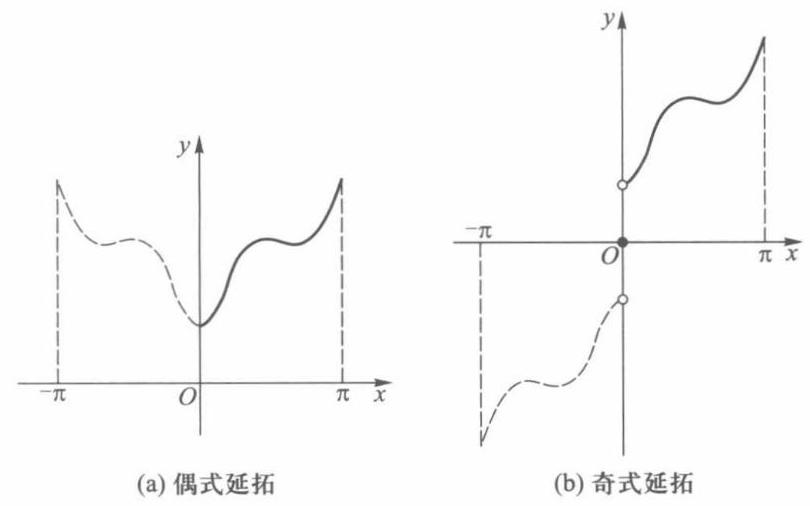
\includegraphics[width=.3\textwidth]{images/P112.jpg}
	\caption{图 $15-8$}
	\label{fig:P112}
\end{figure}

%例 2
\begin{example}

\end{example}
设函数
\[
f\left( x\right)  = \left| {\sin x}\right| , - \pi  \leq  x < \pi ,
\]
求 \(f\) 的傅里叶级数展开式.

%解
\begin{solution}

\end{solution}
\(f\) 是 \(\left\lbrack  {-\pi ,\pi }\right\rbrack\) 上的偶函数,图 15-9 是这函数及其周期延拓的图形. 由于 \(f\) 是按段光滑函数, 因此可以展开成傅里叶级数, 而且这个级数为余弦级数. 由 (10) 式 (这时可把其中“ \~ ”改为“ = ”)知
\[
\left| {\sin x}\right|  = \frac{{a}_{0}}{2} + \mathop{\sum }\limits_{{n = 1}}^{\infty }{a}_{n}\cos {nx},
\]
其中
\[
{a}_{0} = \frac{2}{\pi }{\int }_{0}^{\pi }\sin x\mathrm{\;d}x = \frac{4}{\pi },
\]
\[
{a}_{1} = \frac{2}{\pi }{\int }_{0}^{\pi }\sin x\cos x\mathrm{\;d}x = 0,
\]
\[
{a}_{n} = \frac{2}{\pi }{\int }_{0}^{\pi }\left| {\sin x}\right| \cos {nx}\mathrm{\;d}x = \frac{2}{\pi }{\int }_{0}^{\pi }\sin x\cos {nx}\mathrm{\;d}x
\]
\[
= \frac{2}{\pi }{\int }_{0}^{\pi }\frac{1}{2}\left\lbrack  {\sin \left( {1 - n}\right) x + \sin \left( {1 + n}\right) x}\right\rbrack  \mathrm{d}x
\]
\[
= \frac{1}{\pi }\frac{2}{{n}^{2} - 1}\left\lbrack  {\cos \left( {n - 1}\right) \pi  - 1}\right\rbrack  \;\left( {n \neq  1}\right)
\]
\[
= \left\{  \begin{matrix} 0, & n = 3,5,\cdots , \\   - \frac{4}{\pi }\frac{1}{{n}^{2} - 1}, & n = 2,4,\cdots . \end{matrix}\right.
\]
\begin{figure}
	\centering
	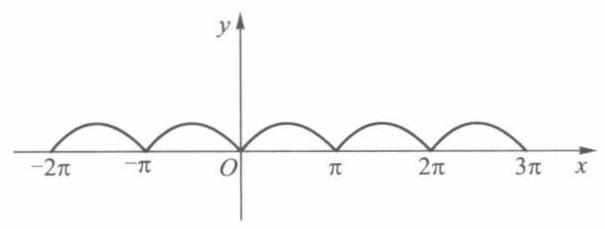
\includegraphics[width=.3\textwidth]{images/P113.jpg}
	\caption{图 $15-9$}
	\label{fig:P113}
\end{figure}

因此
\[
\left| {\sin x}\right|  = \frac{2}{\pi } - \frac{1}{\pi }\mathop{\sum }\limits_{{m = 1}}^{\infty }\frac{4}{4{m}^{2} - 1}\cos {2mx}
\]
\[
= \frac{2}{\pi }\left( {1 - 2\mathop{\sum }\limits_{{m = 1}}^{\infty }\frac{\cos {2mx}}{4{m}^{2} - 1}}\right) , - \infty  < x <  + \infty .
\]
当 \(x = 0\) 时,有
\[
0 = \frac{2}{\pi }\left( {1 - 2\mathop{\sum }\limits_{{m = 1}}^{\infty }\frac{1}{4{m}^{2} - 1}}\right) .
\]
由此可得
\[
\frac{1}{2} = \frac{1}{1 \cdot  3} + \frac{1}{3 \cdot  5} + \cdots  + \frac{1}{\left( {{2m} - 1}\right) \left( {{2m} + 1}\right) } + \cdots .
\]
%例 3
\begin{example}

\end{example}
把定义在 \(\left\lbrack  {0,\pi }\right\rbrack\) 上的函数
\[
f\left( x\right)  = \left\{  \begin{array}{ll} 1, & 0 \leq  x < h, \\  \frac{1}{2}, & x = h, \\  0, & h < x \leq  \pi  \end{array}\right.
\]
(其中 \(0 < h < \pi\) ) 展开成正弦级数.

%解
\begin{solution}

\end{solution}
函数 \(f\) 如图 15-10 所示,它是按段光滑函数,因而可以展开成正弦级数 (12), 其系数
\[
{b}_{n} = \frac{2}{\pi }{\int }_{0}^{\pi }f\left( x\right) \sin {nx}\mathrm{\;d}x = \frac{2}{\pi }{\int }_{0}^{h}\sin {nx}\mathrm{\;d}x
\]
\[
= {\left. \frac{2}{\pi }\left( \frac{-\cos {nx}}{n}\right) \right| }_{0}^{h} = \frac{2}{n\pi }\left( {1 - \cos {nh}}\right) .
\]
所以
\[
f\left( x\right)  = \frac{2}{\pi }\mathop{\sum }\limits_{{n = 1}}^{\infty }\frac{\left( 1 - \cos nh\right) }{n}\sin {nx},\;0 < x < h,\;h < x < \pi .
\]
当 \(x = 0\) 时,级数的和为 0 ; 当 \(x = h\) 时,有
\[
\frac{2}{\pi }\mathop{\sum }\limits_{{n = 1}}^{\infty }\frac{\left( 1 - \cos nh\right) }{n}\sin {nh} = \frac{1 + 0}{2} = \frac{1}{2}.
\]
本题中若 \(h = \pi\) ,则有
\[
f\left( x\right)  = \frac{2}{\pi }\mathop{\sum }\limits_{{n = 1}}^{\infty }\frac{1 - {\left( -1\right) }^{n}}{n}\sin {nx}
\]
\[
= \frac{4}{\pi }\left( {\sin x + \frac{1}{3}\sin {3x} + \frac{1}{5}\sin {5x} + \cdots }\right) ,0 < x < \pi \text{ , }
\]
而且当 \(x = 0,\pi\) 时,级数收敛于 0 .

\begin{figure}
	\centering
	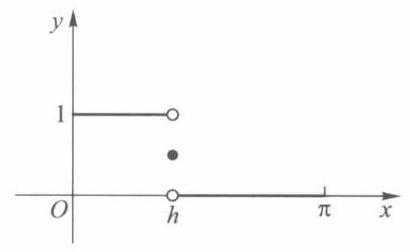
\includegraphics[width=.3\textwidth]{images/P114.jpg}
	\caption{图 $15-10$}
	\label{fig:P114}
\end{figure}

\begin{figure}
	\centering
	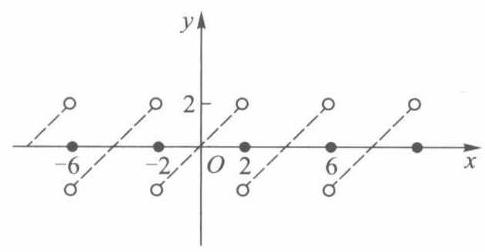
\includegraphics[width=.3\textwidth]{images/P115.jpg}
	\caption{图 $15-11$}
	\label{fig:P115}
\end{figure}

%例 4
\begin{example}

\end{example}
把 \(f\left( x\right)  = x\) 在(0,2)上展开成:

(i) 正弦级数;

(ii) 余弦级数.

%解
\begin{solution}

\end{solution}
(i) 为了要把 \(f\) 展开为正弦级数,对 \(f\) 作奇式周期延拓 (图 15-11),并由公式 (8)有
\[
{a}_{n} = 0,\;n = 0,1,2,\cdots ,
\]
\[
{b}_{n} = \frac{2}{2}{\int }_{0}^{2}x\sin \frac{n\pi x}{2}\mathrm{\;d}x =  - \frac{4}{n\pi }\cos {n\pi } = \frac{4}{n\pi }{\left( -1\right) }^{n + 1},\;n = 1,2,\cdots .
\]
所以当 \(x \in  \left( {0,2}\right)\) 时,由公式 (9) 及收敛定理得到
\[
f\left( x\right)  = x = \mathop{\sum }\limits_{{n = 1}}^{\infty }\frac{4}{n\pi }{\left( -1\right) }^{n + 1}\sin \frac{n\pi x}{2}
\]
\[
= \frac{4}{\pi }\left( {\sin \frac{\pi x}{2} - \frac{1}{2}\sin \frac{2\pi x}{2} + \frac{1}{3}\sin \frac{3\pi x}{2} + \cdots }\right) . \tag{14}
\]
但当 \(x = 0,2\) 时,右边级数收敛于 0 .

(ii) 为了要把 \(f\) 展开为余弦级数,对 \(f\) 作偶式周期延拓 (图 15-12). 由公式 (6) 得 \(f\) 的傅里叶系数为
\[
{b}_{n} = 0,\;n = 1,2,\cdots ,
\]
\[
{a}_{0} = {\int }_{0}^{2}x\mathrm{\;d}x = 2,
\]

\[
{a}_{n} = \frac{2}{2}{\int }_{0}^{2}x\cos \frac{n\pi x}{2}\mathrm{\;d}x = \frac{4}{{n}^{2}{\pi }^{2}}\left( {\cos {n\pi } - 1}\right)
\]
\[
= \frac{4}{{n}^{2}{\pi }^{2}}\left\lbrack  {{\left( -1\right) }^{n} - 1}\right\rbrack  ,\;n = 1,2,\cdots
\]
\begin{figure}
	\centering
	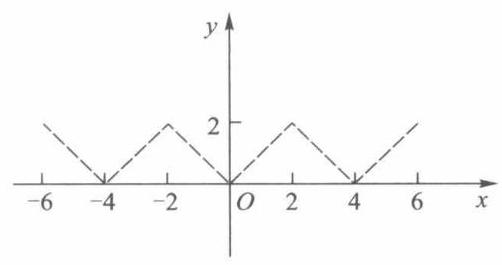
\includegraphics[width=.3\textwidth]{images/P116.jpg}
	\caption{图 $15-12$}
	\label{fig:P116}
\end{figure}

或
\[
{a}_{{2k} - 1} = \frac{-8}{{\left( 2k - 1\right) }^{2}{\pi }^{2}},\;{a}_{2k} = 0\left( {k = 1,2,\cdots }\right) .
\]
所以当 \(x \in  \left( {0,2}\right)\) 时,由公式 (7) 及收敛定理得到
\[
f\left( x\right)  = x = 1 + \mathop{\sum }\limits_{{k = 1}}^{\infty }\frac{-8}{{\left( 2k - 1\right) }^{2}{\pi }^{2}}\cos \frac{\left( {{2k} - 1}\right) {\pi x}}{2}
\]
\[
= 1 - \frac{8}{{\pi }^{2}}\left( {\cos \frac{\pi x}{2} + \frac{1}{{3}^{2}}\cos \frac{3\pi x}{2} + \frac{1}{{5}^{2}}\cos \frac{5\pi x}{2} + \cdots }\right) . \tag{15}
\]
读者由例 4 可以看到, 同样一个函数在同样的区间上可以用正弦级数表示, 也可以用余弦级数表示, 甚至作适当延拓后, 可以用更一般的形式 (5) 来表示.

\subsection{习题 15.2}

1. 求下列周期函数的傅里叶级数展开式:

(1) \(f\left( x\right)  = \left| {\cos x}\right|\) (周期 \(\pi\) )； (2) \(f\left( x\right)  = x - \left\lbrack  x\right\rbrack\) (周期 1)；

(3) \(f\left( x\right)  = {\sin }^{4}x\) (周期 \(\pi\) ); (4) \(f\left( x\right)  = \operatorname{sgn}\left( {\cos x}\right)\) (周期 \({2\pi }\) ).

2. 求函数
\[
f\left( x\right)  = \left\{  \begin{matrix} x, & 0 \leq  x \leq  1, \\  1, & 1 < x < 2, \\  3 - x, & 2 \leq  x \leq  3 \end{matrix}\right.
\]
的傅里叶级数并讨论其敛散性.

3. 将函数 \(f\left( x\right)  = \frac{\pi }{2} - x\) 在 \(\left\lbrack  {0,\pi }\right\rbrack\) 上展开成余弦级数.

4. 将函数 \(f\left( x\right)  = \cos \frac{x}{2}\) 在 \(\left\lbrack  {0,\pi }\right\rbrack\) 上展开成正弦级数.

5. 把函数
\[
f\left( x\right)  = \left\{  \begin{array}{ll} 1 - x, & 0 < x \leq  2, \\  x - 3, & 2 < x < 4 \end{array}\right.
\]
在(0,4)上展开成余弦级数.

6. 把函数 \(f\left( x\right)  = {\left( x - 1\right) }^{2}\) 在(0,1)上展开成余弦级数,并推出
\[
{\pi }^{2} = 6\left( {1 + \frac{1}{{2}^{2}} + \frac{1}{{3}^{2}} + \cdots }\right) .
\]
7. 求下列函数的傅里叶级数展开式:

(1) \(f\left( x\right)  = \arcsin \left( {\sin x}\right)\) ;

(2) \(f\left( x\right)  = \arcsin \left( {\cos x}\right)\) .

8. 试问如何把定义在 \(\left\lbrack  {0,\frac{\pi }{2}}\right\rbrack\) 上的可积函数 \(f\) 延拓到区间 \(\left( {-\pi ,\pi }\right)\) 上,使它们的傅里叶级数为如下的形式:

(1) \(\mathop{\sum }\limits_{{n = 1}}^{\infty }{a}_{{2n} - 1}\cos \left( {{2n} - 1}\right) x\) (2) \(\mathop{\sum }\limits_{{n = 1}}^{\infty }{b}_{{2n} - 1}\sin \left( {{2n} - 1}\right) x\) .

\section{收敛定理的证明}

为了证明傅里叶级数的收敛定理, 先证明下面两个预备定理.

预备定理 1 (贝塞尔 (Bessel) 不等式) 若函数 \(f\) 在 \(\left\lbrack  {-\pi ,\pi }\right\rbrack\) 上可积,则
\[
\frac{{a}_{0}^{2}}{2} + \mathop{\sum }\limits_{{n = 1}}^{\infty }\left( {{a}_{n}^{2} + {b}_{n}^{2}}\right)  \leq  \frac{1}{\pi }{\int }_{-\pi }^{\pi }{f}^{2}\left( x\right) \mathrm{d}x, \tag{1}
\]
其中 \({a}_{n},{b}_{n}\) 为 \(f\) 的傅里叶系数. (1) 式称为贝塞尔不等式.

%证
\begin{proof}

\end{proof}
令
\[
{S}_{m}\left( x\right)  = \frac{{a}_{0}}{2} + \mathop{\sum }\limits_{{n = 1}}^{m}\left( {{a}_{n}\cos {nx} + {b}_{n}\sin {nx}}\right) .
\]
考察积分
\[
{\int }_{-\pi }^{\pi }{\left\lbrack  f\left( x\right)  - {S}_{m}\left( x\right) \right\rbrack  }^{2}\mathrm{\;d}x
\]
\[
= {\int }_{-\pi }^{\pi }{f}^{2}\left( x\right) \mathrm{d}x - 2{\int }_{-\pi }^{\pi }f\left( x\right) {S}_{m}\left( x\right) \mathrm{d}x + {\int }_{-\pi }^{\pi }{S}_{m}^{2}\left( x\right) \mathrm{d}x. \tag{2}
\]
由于
\[
{\int }_{-\pi }^{\pi }f\left( x\right) {S}_{m}\left( x\right) \mathrm{d}x
\]
\[
= \frac{{a}_{0}}{2}{\int }_{-\pi }^{\pi }f\left( x\right) \mathrm{d}x + \mathop{\sum }\limits_{{n = 1}}^{m}\left( {{a}_{n}{\int }_{-\pi }^{\pi }f\left( x\right) \cos {nx}\mathrm{\;d}x + {b}_{n}{\int }_{-\pi }^{\pi }f\left( x\right) \sin {nx}\mathrm{\;d}x}\right) .
\]
根据傅里叶系数公式 \(\left( {§1\text{ ,公式 (10) }}\right)\) 可得
\[
{\int }_{-\pi }^{\pi }f\left( x\right) {S}_{m}\left( x\right) \mathrm{d}x = \frac{\pi }{2}{a}_{0}^{2} + \pi \mathop{\sum }\limits_{{n = 1}}^{m}\left( {{a}_{n}^{2} + {b}_{n}^{2}}\right) . \tag{3}
\]
对于 \({S}_{m}^{2}\left( x\right)\) 的积分,应用三角函数的正交性,有
\[
{\int }_{-\pi }^{\pi }{S}_{m}^{2}\left( x\right) \mathrm{d}x
\]
\[
= {\int }_{-\pi }^{\pi }{\left\lbrack  \frac{{a}_{0}}{2} + \mathop{\sum }\limits_{{n = 1}}^{m}\left( {a}_{n}\cos nx + {b}_{n}\sin nx\right) \right\rbrack  }^{2}\mathrm{\;d}x
\]
\[
= {\left( \frac{{a}_{0}}{2}\right) }^{2}{\int }_{-\pi }^{\pi }\mathrm{d}x + \mathop{\sum }\limits_{{n = 1}}^{m}\left\lbrack  {{a}_{n}^{2}{\int }_{-\pi }^{\pi }{\cos }^{2}{nx}\mathrm{\;d}x + {b}_{n}^{2}{\int }_{-\pi }^{\pi }{\sin }^{2}{nx}\mathrm{\;d}x}\right\rbrack
\]
\[
= \frac{\pi {a}_{0}^{2}}{2} + \pi \mathop{\sum }\limits_{{n = 1}}^{m}\left( {{a}_{n}^{2} + {b}_{n}^{2}}\right) . \tag{4}
\]
将(3)式、(4)式代入(2)式,可得
\[
0 \leq  {\int }_{-\pi }^{\pi }{\left\lbrack  f\left( x\right)  - {S}_{m}\left( x\right) \right\rbrack  }^{2}\mathrm{\;d}x
\]
\[
= {\int }_{-\pi }^{\pi }{f}^{2}\left( x\right) \mathrm{d}x - \frac{\pi {a}_{0}^{2}}{2} - \pi \mathop{\sum }\limits_{{n = 1}}^{m}\left( {{a}_{n}^{2} + {b}_{n}^{2}}\right) .
\]
因而
\[
\frac{{a}_{0}^{2}}{2} + \mathop{\sum }\limits_{{n = 1}}^{m}\left( {{a}_{n}^{2} + {b}_{n}^{2}}\right)  \leq  \frac{1}{\pi }{\int }_{-\pi }^{\pi }{\left\lbrack  f\left( x\right) \right\rbrack  }^{2}\mathrm{\;d}x
\]
对任何正整数 \(m\) 成立. 而 \(\frac{1}{\pi }{\int }_{-\pi }^{\pi }{\left\lbrack  f\left( x\right) \right\rbrack  }^{2}\mathrm{\;d}x\) 为有限值,所以正项级数
\[
\frac{{a}_{0}^{2}}{2} + \mathop{\sum }\limits_{{n = 1}}^{\infty }\left( {{a}_{n}^{2} + {b}_{n}^{2}}\right)
\]
的部分和数列有界, 因而它收敛且有不等式 (1) 成立.

推论 1 若 \(f\) 为可积函数,则
\[
\left. \begin{array}{l} \mathop{\lim }\limits_{{n \rightarrow  \infty }}{\int }_{-\pi }^{\pi }f\left( x\right) \cos {nx}\mathrm{\;d}x = 0, \\  \mathop{\lim }\limits_{{n \rightarrow  \infty }}{\int }_{-\pi }^{\pi }f\left( x\right) \sin {nx}\mathrm{\;d}x = 0. \end{array}\right\}   \tag{5}
\]
因为 (1) 式的左边级数收敛,所以当 \(n \rightarrow  \infty\) 时,通项 \({a}_{n}^{2} + {b}_{n}^{2} \rightarrow  0\) ,亦即有 \({a}_{n} \rightarrow  0\) 与 \({b}_{n} \rightarrow  0\) ,这就是 (5) 式. 这个推论也称为黎曼-勒贝格定理.

推论 2 若 \(f\) 为可积函数,则
\[
\left. \begin{array}{l} \mathop{\lim }\limits_{{n \rightarrow  \infty }}{\int }_{0}^{\pi }f\left( x\right) \sin \left( {n + \frac{1}{2}}\right) x\mathrm{\;d}x = 0, \\  \mathop{\lim }\limits_{{n \rightarrow  \infty }}{\int }_{-\pi }^{0}f\left( x\right) \sin \left( {n + \frac{1}{2}}\right) x\mathrm{\;d}x = 0. \end{array}\right\}   \tag{6}
\]
%证
\begin{proof}

\end{proof}
由于
\[
\sin \left( {n + \frac{1}{2}}\right) x = \cos \frac{x}{2}\sin {nx} + \sin \frac{x}{2}\cos {nx},
\]
所以
\[
{\int }_{0}^{\pi }f\left( x\right) \sin \left( {n + \frac{1}{2}}\right) x\mathrm{\;d}x
\]
\[
= {\int }_{0}^{\pi }\left\lbrack  {f\left( x\right) \cos \frac{x}{2}}\right\rbrack  \sin {nx}\mathrm{\;d}x + {\int }_{0}^{\pi }\left\lbrack  {f\left( x\right) \sin \frac{x}{2}}\right\rbrack  \cos {nx}\mathrm{\;d}x
\]
\[
= {\int }_{-\pi }^{\pi }{F}_{1}\left( x\right) \sin {nx}\mathrm{\;d}x + {\int }_{-\pi }^{\pi }{F}_{2}\left( x\right) \cos {nx}\mathrm{\;d}x\text{ , } \tag{7}
\]
其中
\[
{F}_{1}\left( x\right)  = \left\{  \begin{matrix} f\left( x\right) \cos \frac{x}{2}, & 0 \leq  x \leq  \pi , \\  0, &  - \pi  \leq  x < 0, \end{matrix}\right.
\]
\[
{F}_{2}\left( x\right)  = \left\{  \begin{matrix} f\left( x\right) \sin \frac{x}{2}, & 0 \leq  x \leq  \pi , \\  0, &  - \pi  \leq  x < 0. \end{matrix}\right.
\]
显见 \({F}_{1}\) 与 \({F}_{2}\) 和 \(f\) 一样在 \(\left\lbrack  {-\pi ,\pi }\right\rbrack\) 上可积. 由推论 1,(7) 式右端两积分的极限在 \(n \rightarrow  \infty\) 时都等于零, 所以左边的极限为零.

同样可以证明
\[
\mathop{\lim }\limits_{{n \rightarrow  \infty }}{\int }_{-\pi }^{0}f\left( x\right) \sin \left( {n + \frac{1}{2}}\right) x\mathrm{\;d}x = 0. \tag{0}
\]
预备定理 2 若 \(f\left( x\right)\) 是以 \({2\pi }\) 为周期的函数,且在 \(\left\lbrack  {-\pi ,\pi }\right\rbrack\) 上可积,则它的傅里叶级数部分和 \({S}_{n}\left( x\right)\) 可写成
\[
{S}_{n}\left( x\right)  = \frac{1}{\pi }{\int }_{-\pi }^{\pi }f\left( {x + t}\right) \frac{\sin \left( {n + \frac{1}{2}}\right) t}{2\sin \frac{t}{2}}\mathrm{\;d}t, \tag{8}
\]
当 \(t = 0\) 时,被积函数中的不定式由极限
\[
\mathop{\lim }\limits_{{t \rightarrow  0}}\frac{\sin \left( {n + \frac{1}{2}}\right) t}{2\sin \frac{t}{2}} = n + \frac{1}{2}
\]
来确定.

%证
\begin{proof}

\end{proof}
在傅里叶级数部分和
\[
{S}_{n}\left( x\right)  = \frac{{a}_{0}}{2} + \mathop{\sum }\limits_{{k = 1}}^{n}\left( {{a}_{k}\cos {kx} + {b}_{k}\sin {kx}}\right)
\]
中, 用傅里叶系数公式代入, 可得
\[
{S}_{n}\left( x\right)  = \frac{1}{2\pi }{\int }_{-\pi }^{\pi }f\left( u\right) \mathrm{d}u + \frac{1}{\pi }\mathop{\sum }\limits_{{k = 1}}^{n}\left\lbrack  {\left( {{\int }_{-\pi }^{\pi }f\left( u\right) \cos {ku}\mathrm{\;d}u}\right) \cos {kx} + \left( {{\int }_{-\pi }^{\pi }f\left( u\right) \sin {ku}\mathrm{\;d}u}\right) \sin {kx}}\right\rbrack
\]
\[
= \frac{1}{\pi }{\int }_{-\pi }^{\pi }f\left( u\right) \left\lbrack  {\frac{1}{2} + \mathop{\sum }\limits_{{k = 1}}^{n}\left( {\cos {ku}\cos {kx} + \sin {ku}\sin {kx}}\right) }\right\rbrack  \mathrm{d}u
\]
\[
= \frac{1}{\pi }{\int }_{-\pi }^{\pi }f\left( u\right) \left\lbrack  {\frac{1}{2} + \mathop{\sum }\limits_{{k = 1}}^{n}\cos k\left( {u - x}\right) }\right\rbrack  \mathrm{d}u.
\]
令 \(u = x + t\) ,得
\[
{S}_{n}\left( x\right)  = \frac{1}{\pi }{\int }_{-\pi  - x}^{\pi  - x}f\left( {x + t}\right) \left\lbrack  {\frac{1}{2} + \mathop{\sum }\limits_{{k = 1}}^{n}\cos {kt}}\right\rbrack  \mathrm{d}t.
\]
由上面这个积分看到,被积函数是周期为 \({2\pi }\) 的函数,因此在 \(\left\lbrack  {-\pi  - x,\pi  - x}\right\rbrack\) 上的积分等于 \(\left\lbrack  {-\pi ,\pi }\right\rbrack\) 上的积分,再由第十二章 §3 的 (21) 式,即
\[
\frac{1}{2} + \mathop{\sum }\limits_{{k = 1}}^{n}\cos {kt} = \frac{\sin \left( {n + \frac{1}{2}}\right) t}{2\sin \frac{t}{2}}, \tag{9}
\]
就得到
\[
{S}_{n}\left( x\right)  = \frac{1}{\pi }{\int }_{-\pi }^{\pi }f\left( {x + t}\right) \frac{\sin \left( {n + \frac{1}{2}}\right) t}{2\sin \frac{t}{2}}\mathrm{\;d}t.
\]
(8)式也称为 \(f\) 的傅里叶级数部分和的积分表示式.

现在证明定理 15.3 (收敛定理), 重述如下:

若以 \({2\pi }\) 为周期的函数 \(f\) 在 \(\left\lbrack  {-\pi ,\pi }\right\rbrack\) 上按段光滑,则在每一点 \(x \in  \left\lbrack  {-\pi ,\pi }\right\rbrack  ,f\) 的傅里叶级数 (本章 §1 的 (12) 式) 收敛于 \(f\) 在点 \(x\) 的左、右极限的算术平均值,即
\[
\frac{f\left( {x + 0}\right)  + f\left( {x - 0}\right) }{2} = \frac{{a}_{0}}{2} + \mathop{\sum }\limits_{{n = 1}}^{\infty }\left( {{a}_{n}\cos {nx} + {b}_{n}\sin {nx}}\right) ,
\]
其中 \({a}_{n},{b}_{n}\) 为 \(f\) 的傅里叶系数.

%证
\begin{proof}

\end{proof}
只要证明在每一点 \(x\) 处下述极限成立:
\[
\mathop{\lim }\limits_{{n \rightarrow  \infty }}\left\lbrack  {\frac{f\left( {x + 0}\right)  + f\left( {x - 0}\right) }{2} - {S}_{n}\left( x\right) }\right\rbrack   = 0,
\]
即
\[
\mathop{\lim }\limits_{{n \rightarrow  \infty }}\left\lbrack  {\frac{f\left( {x + 0}\right)  + f\left( {x - 0}\right) }{2} - \frac{1}{\pi }{\int }_{-\pi }^{\pi }f\left( {x + t}\right) \frac{\sin \left( {n + \frac{1}{2}}\right) t}{2\sin \frac{t}{2}}\mathrm{\;d}t}\right\rbrack   = 0,
\]
或证明同时有
\[
\mathop{\lim }\limits_{{n \rightarrow  \infty }}\left\lbrack  {\frac{f\left( {x + 0}\right) }{2} - \frac{1}{\pi }{\int }_{0}^{\pi }f\left( {x + t}\right) \frac{\sin \left( {n + \frac{1}{2}}\right) t}{2\sin \frac{t}{2}}\mathrm{\;d}t}\right\rbrack   = 0 \tag{10}
\]
与
\[
\mathop{\lim }\limits_{{n \rightarrow  \infty }}\left\lbrack  {\frac{f\left( {x - 0}\right) }{2} - \frac{1}{\pi }{\int }_{-\pi }^{0}f\left( {x + t}\right) \frac{\sin \left( {n + \frac{1}{2}}\right) t}{2\sin \frac{t}{2}}\mathrm{\;d}t}\right\rbrack   = 0. \tag{11}
\]
现在先证明 (10) 式. 对 (9) 式积分有
\[
\frac{1}{\pi }{\int }_{-\pi }^{\pi }\frac{\sin \left( {n + \frac{1}{2}}\right) t}{2\sin \frac{t}{2}}\mathrm{\;d}t = \frac{1}{\pi }{\int }_{-\pi }^{\pi }\left( {\frac{1}{2} + \mathop{\sum }\limits_{{k = 1}}^{n}\cos {kt}}\right) \mathrm{d}t = 1.
\]
由于上式左边为偶函数,因此两边乘以 \(f\left( {x + 0}\right)\) 后得到
\[
\frac{f\left( {x + 0}\right) }{2} = \frac{1}{\pi }{\int }_{0}^{\pi }f\left( {x + 0}\right) \frac{\sin \left( {n + \frac{1}{2}}\right) t}{2\sin \frac{t}{2}}\mathrm{\;d}t.
\]
从而 (10) 式可改写为
\[
\mathop{\lim }\limits_{{n \rightarrow  \infty }}\frac{1}{\pi }{\int }_{0}^{\pi }\left\lbrack  {f\left( {x + 0}\right)  - f\left( {x + t}\right) }\right\rbrack  \frac{\sin \left( {n + \frac{1}{2}}\right) t}{2\sin \frac{t}{2}}\mathrm{\;d}t = 0. \tag{12}
\]
令
\[
\varphi \left( t\right)  =  - \frac{f\left( {x + t}\right)  - f\left( {x + 0}\right) }{2\sin \frac{t}{2}}
\]
\[
=  - \left\lbrack  \frac{f\left( {x + t}\right)  - f\left( {x + 0}\right) }{t}\right\rbrack  \frac{\frac{t}{2}}{\sin \frac{t}{2}},\;t \in  (0,\pi \rbrack .
\]
由本章 §1 的(13)式得
\[
\mathop{\lim }\limits_{{t \rightarrow  {0}^{ + }}}\varphi \left( t\right)  =  - {f}^{\prime }\left( {x + 0}\right)  \cdot  1 =  - {f}^{\prime }\left( {x + 0}\right) .
\]
再令 \(\varphi \left( 0\right)  =  - {f}^{\prime }\left( {x + 0}\right)\) ,则函数 \(\varphi\) 在点 \(t = 0\) 右连续. 因为 \(\varphi\) 在 \(\left\lbrack  {0,\pi }\right\rbrack\) 上至多只有有限个第一类间断点,所以 \(\varphi\) 在 \(\left\lbrack  {0,\pi }\right\rbrack\) 上可积. 根据预备定理 1 的推论 2,
\[
\mathop{\lim }\limits_{{n \rightarrow  \infty }}\frac{1}{\pi }{\int }_{0}^{\pi }\left\lbrack  {f\left( {x + 0}\right)  - f\left( {x + t}\right) }\right\rbrack  \frac{\sin \left( {n + \frac{1}{2}}\right) t}{2\sin \frac{t}{2}}\mathrm{\;d}t
\]
\[
= \mathop{\lim }\limits_{{n \rightarrow  \infty }}\frac{1}{\pi }{\int }_{0}^{\pi }\varphi \left( t\right) \sin \left( {n + \frac{1}{2}}\right) t\mathrm{\;d}t = 0.
\]
这就证得 (12) 式成立, 从而 (10) 式成立.

用同样方法可证 (11) 式也成立.

\subsection{习题 15.3\footnote{本节习题均为选做题.}}

1. 设 \(f\) 以 \({2\pi }\) 为周期且具有二阶连续的导函数,证明 \(f\) 的傅里叶级数在 \(\left( {-\infty , + \infty }\right)\) 上一致收敛于 \(f\) .

2. 设 \(f\) 为 \(\left\lbrack  {-\pi ,\pi }\right\rbrack\) 上的可积函数. 证明: 若 \(f\) 的傅里叶级数在 \(\left\lbrack  {-\pi ,\pi }\right\rbrack\) 上一致收敛于 \(f\) ,则成立帕塞瓦尔 (Parseval) 等式:
\[
\frac{1}{\pi }{\int }_{-\pi }^{\pi }{\left\lbrack  f\left( x\right) \right\rbrack  }^{2}\mathrm{\;d}x = \frac{{a}_{0}^{2}}{2} + \mathop{\sum }\limits_{{n = 1}}^{\infty }\left( {{a}_{n}^{2} + {b}_{n}^{2}}\right) ,
\]
这里 \({a}_{n},{b}_{n}\) 为 \(f\) 的傅里叶系数.

3. 帕塞瓦尔等式对于在 \(\left\lbrack  {-\pi ,\pi }\right\rbrack\) 上满足收敛定理条件的函数也成立 (证略). 请应用这个结果证明下列各式:

(1) \(\frac{{\pi }^{2}}{8} = \mathop{\sum }\limits_{{n = 1}}^{\infty }\frac{1}{{\left( 2n - 1\right) }^{2}}\) (提示: 应用 §1 习题 3 的展开式导出);

(2) \(\frac{{\pi }^{2}}{6} = \mathop{\sum }\limits_{{n = 1}}^{\infty }\frac{1}{{n}^{2}}\) (提示:应用 §1 习题 1(1)(i)的展开式导出);



(3) \(\frac{{\pi }^{4}}{90} = \mathop{\sum }\limits_{{n = 1}}^{\infty }\frac{1}{{n}^{4}}\) (提示:应用 §1 习题 \(1\left( 2\right)\) (i) 的展开式导出).

4. 证明: 若 \(f,g\) 均为 \(\left\lbrack  {-\pi ,\pi }\right\rbrack\) 上的可积函数,且它们的傅里叶级数在 \(\left\lbrack  {-\pi ,\pi }\right\rbrack\) 上分别一致收敛于 \(f\) 和 \(g\) ,则
\[
\frac{1}{\pi }{\int }_{-\pi }^{\pi }f\left( x\right) g\left( x\right) \mathrm{d}x = \frac{{a}_{0}{\alpha }_{0}}{2} + \mathop{\sum }\limits_{{n = 1}}^{\infty }\left( {{a}_{n}{\alpha }_{n} + {b}_{n}{\beta }_{n}}\right) ,
\]
其中 \({a}_{n},{b}_{n}\) 为 \(f\) 的傅里叶系数, \({\alpha }_{n},{\beta }_{n}\) 为 \(g\) 的傅里叶系数.

5. 证明: 若 \(f\) 及其导函数 \({f}^{\prime }\) 均在 \(\left\lbrack  {-\pi ,\pi }\right\rbrack\) 上可积, \({\int }_{-\pi }^{\pi }f\left( x\right) \mathrm{d}x = 0,f\left( {-\pi }\right)  = f\left( \pi \right)\) ,且成立帕塞瓦尔等式, 则
\[
{\int }_{-\pi }^{\pi }{\left| {f}^{\prime }\left( x\right) \right| }^{2}\mathrm{\;d}x \geq  {\int }_{-\pi }^{\pi }{\left| f\left( x\right) \right| }^{2}\mathrm{\;d}x.
\]
\section{总练习题}

1. 试求三角多项式
\[
{T}_{n}\left( x\right)  = \frac{{A}_{0}}{2} + \mathop{\sum }\limits_{{k = 1}}^{n}\left( {{A}_{k}\cos {kx} + {B}_{k}\sin {kx}}\right)
\]
的傅里叶级数展开式.

2. 设 \(f\) 为 \(\left\lbrack  {-\pi ,\pi }\right\rbrack\) 上的可积函数, \({a}_{0},{a}_{k},{b}_{k}\left( {k = 1,2,\cdots ,n}\right)\) 为 \(f\) 的傅里叶系数. 试证明: 当
\[
{A}_{0} = {a}_{0},\;{A}_{k} = {a}_{k},\;{B}_{k} = {b}_{k}\;\left( {k = 1,2,\cdots ,n}\right)
\]
时, 积分
\[
{\int }_{-\pi }^{\pi }{\left\lbrack  f\left( x\right)  - {T}_{n}\left( x\right) \right\rbrack  }^{2}\mathrm{\;d}x
\]
取最小值, 且最小值为
\[
{\int }_{-\pi }^{\pi }{\left\lbrack  f\left( x\right) \right\rbrack  }^{2}\mathrm{\;d}x - \pi \left\lbrack  {\frac{{a}_{0}^{2}}{2} + \mathop{\sum }\limits_{{k = 1}}^{n}\left( {{a}_{k}^{2} + {b}_{k}^{2}}\right) }\right\rbrack  .
\]
上述 \({T}_{n}\left( x\right)\) 是第 1 题中的三角多项式, \({A}_{0},{A}_{k},{B}_{k}\) 为它的傅里叶系数.

3. 设 \(f\) 是以 \({2\pi }\) 为周期,且具有二阶连续可微的函数,
\[
{b}_{n} = \frac{1}{\pi }{\int }_{-\pi }^{\pi }f\left( x\right) \sin {nx}\mathrm{\;d}x,\;{b}_{n}^{\prime \prime } = \frac{1}{\pi }{\int }_{-\pi }^{\pi }{f}^{\prime \prime }\left( x\right) \sin {nx}\mathrm{\;d}x.
\]
若级数 \(\sum {b}_{n}^{\prime \prime }\) 绝对收敛,则
\[
\mathop{\sum }\limits_{{n = 1}}^{\infty }\sqrt{\left| {b}_{n}\right| } \leq  \frac{1}{2}\left( {2 + \mathop{\sum }\limits_{{n = 1}}^{\infty }\left| {b}_{n}^{\prime \prime }\right| }\right) .
\]
4. 设周期为 \({2\pi }\) 的可积函数 \(\varphi \left( x\right)\) 与 \(\psi \left( x\right)\) 满足以下关系式:

(1) \(\varphi \left( {-x}\right)  = \psi \left( x\right)\) ;

(2) \(\varphi \left( {-x}\right)  =  - \psi \left( x\right)\) .

试问 \(\varphi\) 的傅里叶系数 \({a}_{n},{b}_{n}\) 与 \(\psi\) 的傅里叶系数 \({\alpha }_{n},{\beta }_{n}\) 有什么关系?

5. 设定义在 \(\left\lbrack  {a,b}\right\rbrack\) 上的连续函数列 \(\left\{  {\varphi }_{n}\right\}\) 满足关系
\[
{\int }_{a}^{b}{\varphi }_{n}\left( x\right) {\varphi }_{m}\left( x\right) \mathrm{d}x = \left\{  \begin{array}{ll} 0, & n \neq  m, \\  1, & n = m. \end{array}\right.
\]
对于在 \(\left\lbrack  {a,b}\right\rbrack\) 上的可积函数 \(f\) ,定义
\[
{a}_{n} = {\int }_{a}^{b}f\left( x\right) {\varphi }_{n}\left( x\right) \mathrm{d}x,\;n = 1,2,\cdots .
\]
证明: \(\mathop{\sum }\limits_{{n = 1}}^{\infty }{a}_{n}^{2}\) 收敛,且有不等式
\[
\mathop{\sum }\limits_{{n = 1}}^{\infty }{a}_{n}^{2} \leq  {\int }_{a}^{b}{\left\lbrack  f\left( x\right) \right\rbrack  }^{2}\mathrm{\;d}x.
\]
第十五章综合自测题

